\documentclass[../report.tex]{subfiles}
\graphicspath{{\subfix{../image/}}}

\begin{document}

\subsection{Analog IR-Sensors}
The chosen method of navigation is lines on the floor. To see them, a sensor is necessary.
The market offers a wide range of modules. Both digital and analog. It was decided to go with 
a analog variant for the following reasons: learning experience and custom calibration values -> more
floor types possible (TEKExpo floor is, for example, different from the one in the project room).  

The chosen model combines 8 IR-LEDs with 8 photoresistors. The output is an analog voltage. One for each photoresistor.
The final forklift has two of these arrays. One mounted in the front and one in the back - mounted
close to the floor (see picture). The distance has been determined over several rounds of testing 
including different materials. The number and placement of the arrays allows the forklift to easily detect
how it is placed on the line and to detect intersections.  
\begin{figure}[h!]
    \centering
    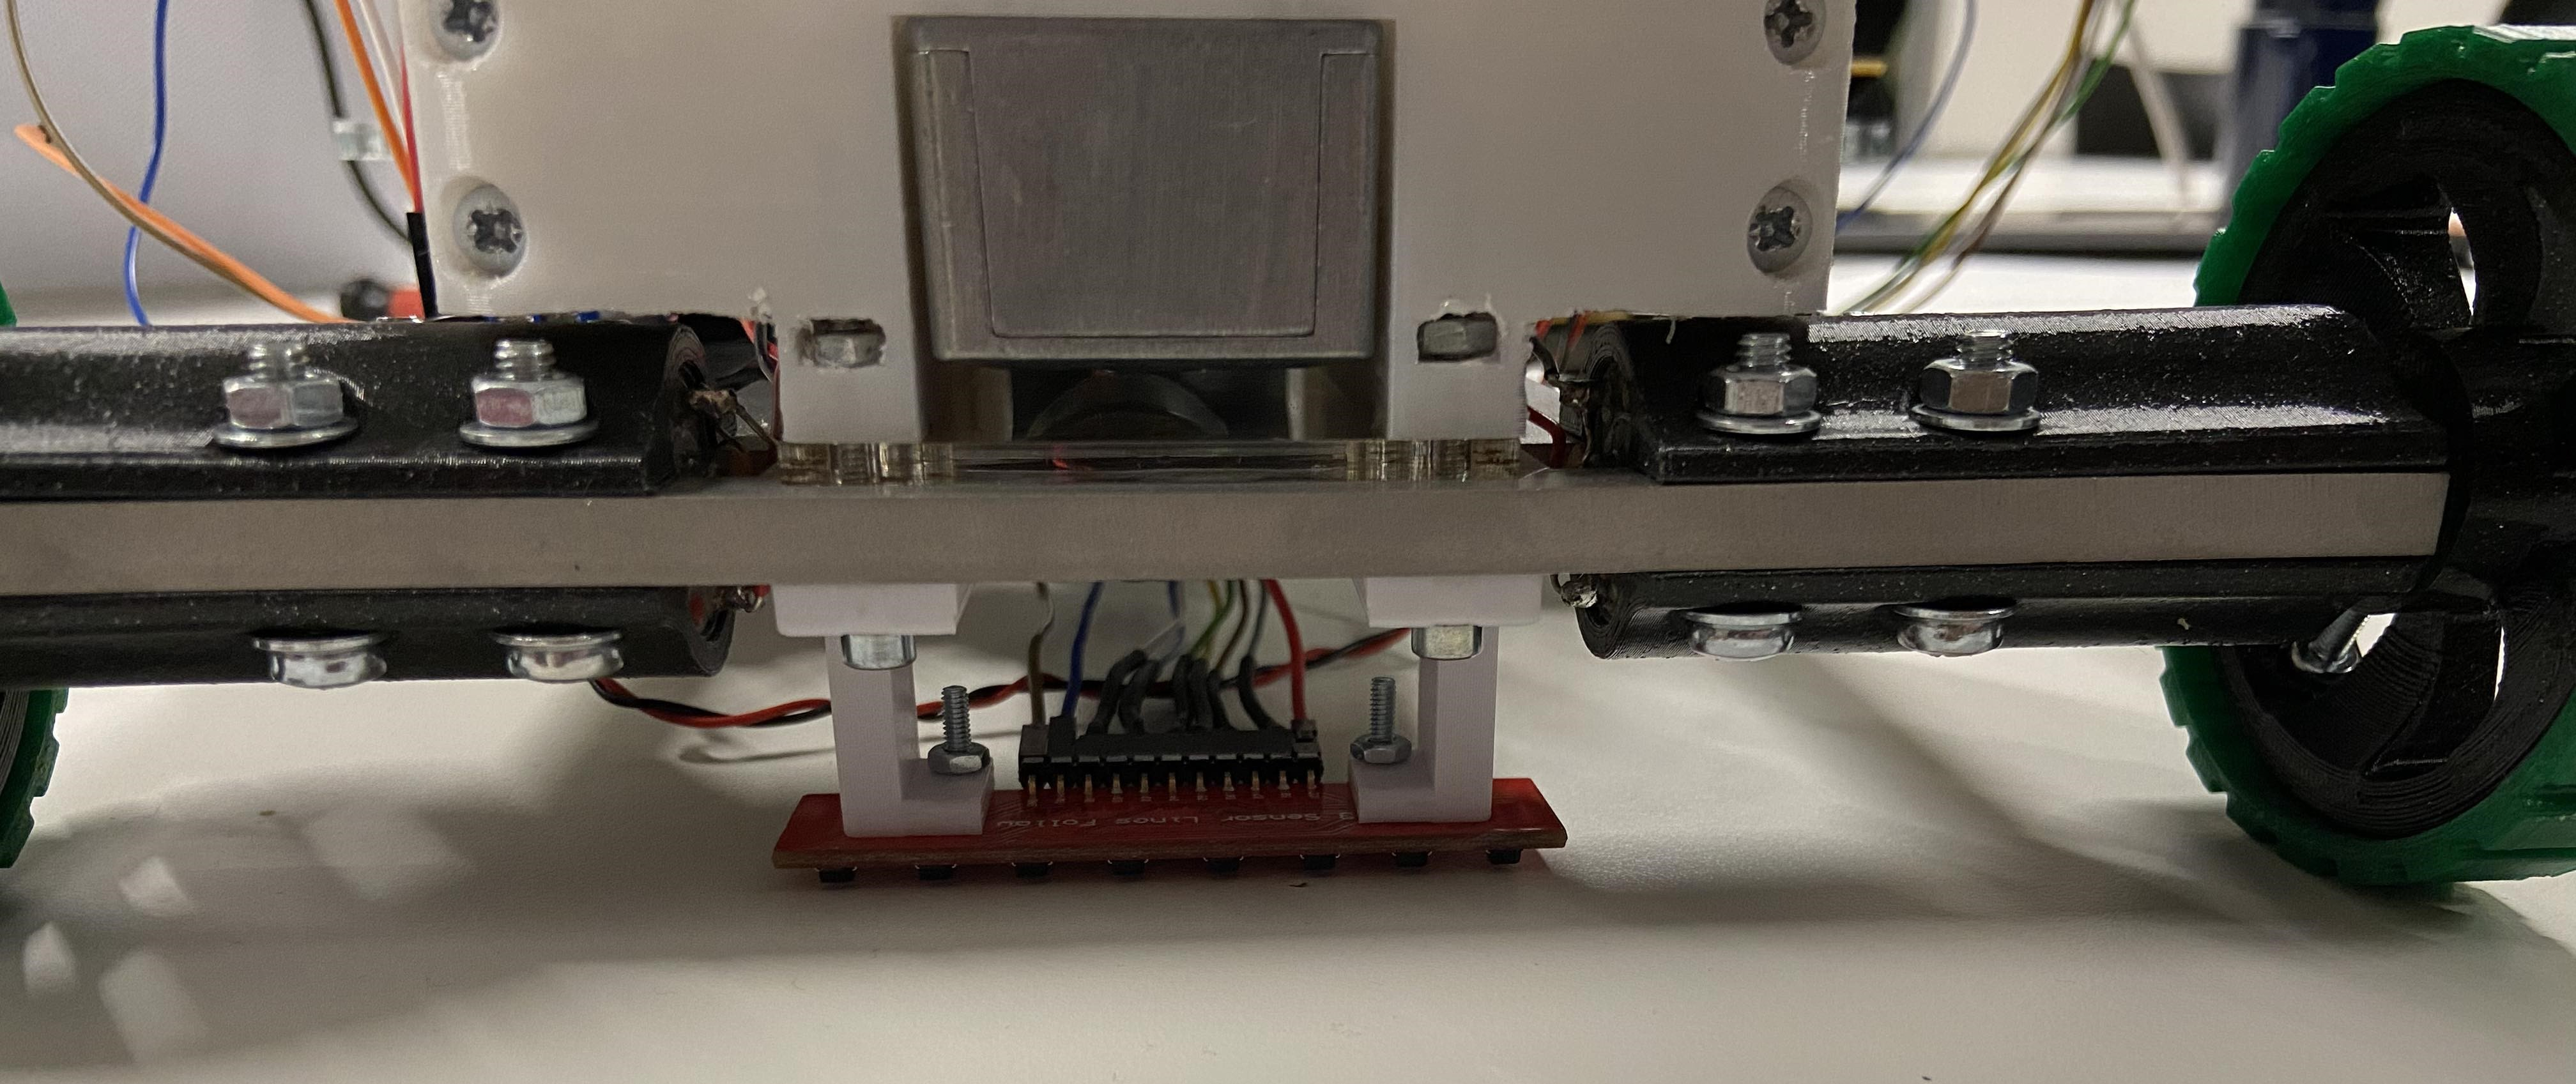
\includegraphics[width=0.2\textwidth]{IRsensorinholder.jpg}
    \caption{One of the IR-sensor arrays in holder}
 \end{figure}

However, using the analog variant requires all of the 16 outputs to be connected to an ADC-pin at some point.
Even though the chosen microcontroller has 18 measurement channels, not all of them are available to use.
For example, about half of all channels can only be used while the WiFi-functionalities of the chip are not used.
Why this is problematic will become clear in the section ``Connectivity and Communication'' in the code section.
Moreover, other pins are simply not available to use, simply because they are shared between ADC and other modules.
Additionally, some ADC pins are also required for monitoring the battery voltage and the weight on the fork.
Consequently, it is impossible to have all of them connected at the same time. However, what cannot be done 
simultaneously can be done sequentially. To see be able to read all the analog outputs multiplexers are used.

\end{document}